% ============================================================
%  Real FFT Architecture on FPGA  –  Corrected Overleaf document
%  Target: Sipeed Tang Primer 20K (Gowin GW2A-LV18PG256C8/I7)
%  Compile with: pdflatex (twice for cross-references)
% ============================================================
\documentclass[12pt, a4paper]{article}

% ---------- Packages (duplicates removed) ----------
\usepackage[T1]{fontenc}
\usepackage[utf8]{inputenc}
\usepackage{lmodern}
\usepackage{microtype}
\usepackage{geometry}
\geometry{margin=2.5cm}
\usepackage{amsmath}
\usepackage{amssymb}
\usepackage{graphicx}
\usepackage{tikz}
\usetikzlibrary{arrows.meta, positioning, shapes.geometric}
\usepackage{hyperref}
\usepackage{booktabs}
\usepackage{longtable}
\usepackage{array}
\usepackage{tabularx}
\usepackage{float}
\usepackage{enumitem}
\usepackage{xcolor}
\usepackage{fancyhdr}
\usepackage{titlesec}
\hypersetup{colorlinks=true, linkcolor=blue, urlcolor=blue}
\graphicspath{{img/}}

% ---------- Title ----------
\title{\textbf{Real FFT Architecture on FPGA}}
\author{}
\date{}

% ============================================================
\begin{document}
\maketitle
\tableofcontents
\newpage

% ------------------------------------------------------------
\section{Real FFT Architecture on FPGA}

% ------------------------------------------------------------
\subsection{Project Overview}

This section describes the hardware architecture of a Real Fast Fourier
Transform (RFFT) implemented on a Sipeed Tang Primer 20K FPGA
(Gowin GW2A-LV18PG256C8/I7).
Rather than running a full $N$-point complex FFT on real-valued data, the
architecture exploits the conjugate-symmetry property of the DFT for real
signals by \emph{packing} the $N = 2048$ real input samples into $N/2 = 1024$
complex samples and running a 1024-point complex FFT core internally.
A final recombination stage then recovers the 1025 unique frequency bins that
constitute the RFFT output.

Because the spectrum of a real sequence satisfies
\begin{equation}
    X[k] = X^{*}[N-k],
\end{equation}
only the first $N/2 + 1 = 1025$ output bins carry unique information.
The packing-plus-recombination strategy halves the internal FFT size compared
with a na\"{i}ve complex implementation, reducing DSP, BRAM, and latency
accordingly.
The target device provides 48 DSP multiplier blocks (18$\times$18) and
828\,Kbits of on-chip block SRAM, making fixed-point arithmetic and
memory-based twiddle-factor storage the natural implementation strategy.

% ------------------------------------------------------------
\subsection{Input Signal and Q15 Representation}

The system accepts a real-valued discrete-time signal $x[n]$ of length
$N = 2048$ sampled at $f_s = 48\,\text{kHz}$.
All data are represented in \emph{Q15} fixed-point format: one sign bit
followed by 15 fractional bits packed into a 16-bit two's-complement word,
giving a dynamic range of $[-1,\,1)$ with a resolution of
$2^{-15} \approx 3.05 \times 10^{-5}$.
This format is well suited to audio signals and normalised twiddle factors,
both of which are bounded within $[-1, 1]$, and it maps directly onto the
DSP multiply-accumulate (MAC) units available in the target FPGA without
requiring a floating-point unit.

The Q15 stream is produced by one of two front-end paths:
\begin{equation}
    \text{Digital mic (I2S)} \;\longrightarrow\;
    \text{I2S deserialiser} \;\longrightarrow\; \text{Q15 stream at }48\,\text{kHz},
\end{equation}
\begin{equation}
    \text{Analogue mic} \;\longrightarrow\;
    \text{16-bit ADC} \;\longrightarrow\; \text{Q15 stream at }48\,\text{kHz}.
\end{equation}

% ------------------------------------------------------------
\subsection{Packing Stage: Real-to-Complex Conversion}

Before the complex FFT core is invoked, the 2048 real samples are packed into
1024 complex samples by interleaving even- and odd-indexed inputs:
\begin{equation}
    z[m] = x[2m] + j\,x[2m+1], \qquad m = 0, 1, \ldots, 1023.
\end{equation}
This is the standard trick that allows a single $N/2$-point complex FFT to
process an $N$-point real sequence.
The packed complex stream $z[m]$ is passed to the 1024-point Radix-2 DIT core
described in Section~\ref{sec:fftcore}.

% ------------------------------------------------------------
\subsection{Twiddle Factor Generation and Storage}

Two sets of twiddle factors are required:
\begin{enumerate}[leftmargin=*, label=\alph*)]
    \item \textbf{FFT twiddle factors} for the 1024-point complex FFT core:
        \begin{equation}
            W_{1024}^{\,k} = \cos\!\left(\frac{2\pi k}{1024}\right)
                           - j\sin\!\left(\frac{2\pi k}{1024}\right),
            \qquad k = 0, 1, \ldots, 511.
        \end{equation}
    \item \textbf{Recombination twiddle factors} for the final RFFT stage
        (Section~\ref{sec:recombine}):
        \begin{equation}
            W_{2048}^{\,k} = \cos\!\left(\frac{2\pi k}{2048}\right)
                           - j\sin\!\left(\frac{2\pi k}{2048}\right),
            \qquad k = 0, 1, \ldots, 1024.
        \end{equation}
\end{enumerate}

Both tables are precomputed offline in Python using double-precision arithmetic
and then quantised to Q15 by multiplying by $2^{15}$ and rounding to the
nearest integer, yielding 16-bit signed integers in the range
$[-32768,\,32767]$.
Each twiddle entry is packed into a single 32-bit ROM word:
\begin{equation}
    \underbrace{\mathrm{Re}\{W^k\}}_{\text{bits }[31:16]}
    \;\|\;
    \underbrace{\mathrm{Im}\{W^k\}}_{\text{bits }[15:0]}.
\end{equation}

The tables are written to \texttt{.mi} memory-initialisation files (Gowin
BSRAM format) and loaded into a single-port ROM synthesised from the on-chip
BSRAM.
The FFT stage controller addresses the FFT twiddle ROM with the appropriate
stage-dependent stride; the recombination stage uses the $W_{2048}^k$ table
directly.

% ------------------------------------------------------------
\subsection{Radix-2 DIT FFT Core}
\label{sec:fftcore}

The internal complex FFT engine is a 1024-point Radix-2
Decimation-in-Time (DIT) core.
The DFT of the packed sequence $z[m]$,
\begin{equation}
    Z[k] = \sum_{m=0}^{1023} z[m]\,W_{1024}^{\,km},
\end{equation}
is recursively decomposed by separating even-indexed and odd-indexed samples:
\begin{equation}
    Z[k] = E[k] + W_{1024}^{\,k}\,O[k],
\end{equation}
where $E[k]$ and $O[k]$ are the 512-point DFTs of the even and odd
sub-sequences of $z[m]$, respectively.
This factorisation is applied $\log_2 1024 = 10$ times, reducing the
operation count from $\mathcal{O}(N^2)$ to $\mathcal{O}(N\log_2 N)$.

Because the DIT algorithm requires bit-reversed input order, a bit-reversal
permutation is applied to the packed data before the first butterfly stage.
The reordering is implemented using the dual-port RAM blocks in the FPGA,
allowing simultaneous read and write access during permutation.
Separate dual-port RAM banks are used for the bit-reversal buffer and for
the inter-stage butterfly pipeline, to avoid address conflicts on the
single-port BSRAM macros.

% ------------------------------------------------------------
\subsection{Butterfly Computation and Scaling}

Each butterfly unit receives an even-indexed term $E[k]$, an odd-indexed
term $O[k]$, and the twiddle factor $W_{1024}^k$ for the current stage,
producing the two output bins
\begin{align}
    Z_\text{out}[k]       &= E[k] + W_{1024}^{\,k}\,O[k], \label{eq:bf_top}\\
    Z_\text{out}[k + N/2] &= E[k] - W_{1024}^{\,k}\,O[k]. \label{eq:bf_bot}
\end{align}

The complex multiplication $W_{1024}^k \cdot O[k]$ expands to four real
multiplications and two additions and is mapped onto the DSP MAC blocks.
In Q15 arithmetic, the product of two 16-bit Q15 numbers produces a 32-bit
Q30 result; a right-shift by 15 bits with symmetric saturation to
\texttt{0x7FFF} / \texttt{0x8000} is applied to restore the Q15 format.
Additionally, a one-bit arithmetic right-shift (divide-by-two) is applied
to both outputs after each butterfly addition to prevent overflow
accumulation across the 10 stages.

\textbf{Scale factor note.}
The combination of the post-multiplication 15-bit shift and the per-stage
1-bit shift introduces a total scale factor of $1/2^{10} = 1/1024$ on the
FFT output relative to an unscaled DFT.
All Python reference models must apply an equivalent $1/1024$ normalisation
(or equivalently, compare using \texttt{numpy.fft.fft()} with the
\texttt{norm="forward"} argument divided by the appropriate power of two)
so that numerical comparisons remain within the $\pm 2$\,LSB tolerance.

% ------------------------------------------------------------
\subsection{RFFT Recombination Stage}
\label{sec:recombine}

After the 1024-point complex FFT produces $Z[k]$, a dedicated recombination
module recovers the 1025 unique bins of the 2048-point real FFT.
Let $Z[k]$ be the output of the complex core.
The recombination equations are:
\begin{align}
    A[k] &= \tfrac{1}{2}\bigl(Z[k] + Z^{*}[1024-k]\bigr), \\
    B[k] &= \tfrac{1}{2}\bigl(Z[k] - Z^{*}[1024-k]\bigr)\cdot(-j), \\
    X[k] &= A[k] + W_{2048}^{\,k}\,B[k],
            \qquad k = 0, 1, \ldots, 1024,
\end{align}
where $Z^{*}$ denotes complex conjugate and $Z[0]$ is used for the boundary
condition $Z[1024] \equiv Z[0]$ (periodicity).
The DC bin $X[0]$ and Nyquist bin $X[1024]$ are purely real and are computed
as special cases:
\begin{align}
    X[0]    &= \mathrm{Re}(Z[0]) + \mathrm{Im}(Z[0]), \\
    X[1024] &= \mathrm{Re}(Z[0]) - \mathrm{Im}(Z[0]).
\end{align}

This recombination stage uses the $W_{2048}^k$ twiddle ROM and must be
validated independently against the Python reference
\texttt{numpy.fft.rfft(x, n=2048)} before integration.

% ------------------------------------------------------------
\subsection{Hardware Processing Flow}

Figure~\ref{fig:rfft_flow} illustrates the end-to-end processing pipeline.

\begin{figure}[ht]
\centering
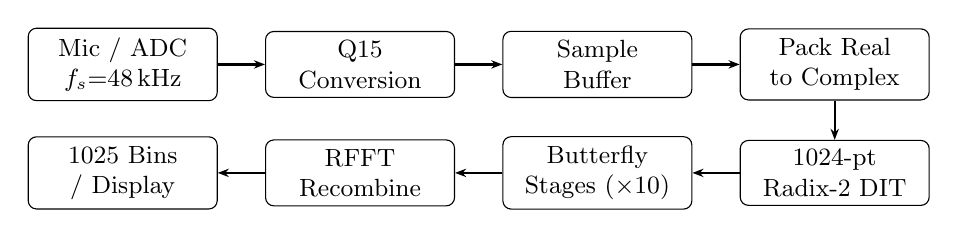
\begin{tikzpicture}[
    node distance = 5mm and 6mm,
    box/.style = {draw, rounded corners=3pt,
                  minimum width=2.4cm, minimum height=0.75cm,
                  align=center, font=\small},
    arr/.style = {-{Stealth[length=4pt]}, thick}
]
    % Row 1 (left to right)
    \node[box] (in)   {Mic / ADC\\$f_s{=}48\,\text{kHz}$};
    \node[box, right=of in]   (q15)  {Q15\\Conversion};
    \node[box, right=of q15]  (buf)  {Sample\\Buffer};
    \node[box, right=of buf]  (pack) {Pack Real\\to Complex};

    % Row 2 (right to left, below row 1)
    \node[box, below=of pack] (dit)  {1024-pt\\Radix-2 DIT};
    \node[box, left=of dit]   (bf)   {Butterfly\\Stages ($\times$10)};
    \node[box, left=of bf]    (rec)  {RFFT\\Recombine};
    \node[box, left=of rec]   (out)  {1025 Bins\\/ Display};

    % Arrows row 1
    \draw[arr] (in)   -- (q15);
    \draw[arr] (q15)  -- (buf);
    \draw[arr] (buf)  -- (pack);

    % Turn down
    \draw[arr] (pack) -- (dit);

    % Arrows row 2
    \draw[arr] (dit) -- (bf);
    \draw[arr] (bf)  -- (rec);
    \draw[arr] (rec) -- (out);
\end{tikzpicture}
\caption{FPGA processing pipeline for the Real FFT implementation.
         The microphone or ADC front-end feeds a 48\,kHz Q15 stream;
         samples are packed into complex pairs before the internal
         1024-point FFT; the recombination stage produces the 1025
         unique bins that are forwarded to the display.}
\label{fig:rfft_flow}
\end{figure}

Figure~\ref{fig:spectrum_fft_spec} shows the provided spectrum FFT
specification diagram, including the global Q15 data format and the major
datapath blocks from input capture through display.

\begin{figure}[H]
\centering
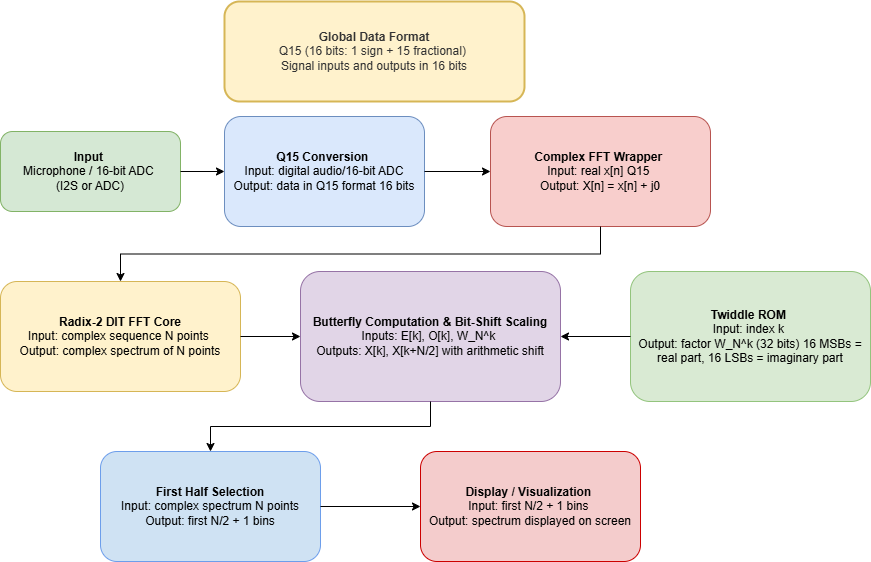
\includegraphics[width=0.95\textwidth]{spectrum_fft_spec.png}
\caption{Spectrum FFT specification block diagram.}
\label{fig:spectrum_fft_spec}
\end{figure}

The input signal is first converted to a 16-bit Q15 stream at 48\,kHz.
The sample buffer collects exactly 2048 samples per frame.
The packing stage maps 2048 real samples to 1024 complex samples
(even$\,\to\,$Re, odd$\,\to\,$Im).
The bit-reversal permutation reorders the packed data, then the
1024-point Radix-2 DIT core executes the 10 butterfly stages, fetching
twiddle factors from the FFT ROM with stage-dependent address strides.
Per-stage 1-bit scaling prevents overflow accumulation.
The recombination module applies the RFFT post-processing equations and
the $W_{2048}^k$ twiddle ROM to recover all 1025 bins, which are forwarded
to the magnitude calculator and the display.

Hardware resources used:
\begin{itemize}[leftmargin=*]
    \item \textbf{Dual-port RAM (BSRAM):} separate banks for the bit-reversal
          permutation buffer and the inter-stage working memory.
    \item \textbf{Single-port ROM (BSRAM):} FFT twiddle table ($W_{1024}^k$,
          $k=0\ldots511$) and recombination twiddle table
          ($W_{2048}^k$, $k=0\ldots1024$), each packed as
          $32$-bit words.
    \item \textbf{DSP slices:} complex multiplications in the butterfly unit
          (4 real multiplies per butterfly) and in the recombination stage.
    \item \textbf{Fixed-point arithmetic:} Q15 throughout; post-multiplication
          shift of 15 bits with saturation; per-stage 1-bit shift with
          total scale factor $1/1024$.
\end{itemize}

% ------------------------------------------------------------
\subsection{Design Summary}

The proposed architecture achieves an efficient FPGA implementation of the
2048-point Real FFT on the Tang Primer 20K by exploiting real-to-complex
packing so that only a 1024-point internal complex FFT core is required.
Offline precomputation of twiddle factors in Python eliminates run-time
trigonometric operations and confines the on-chip computation to integer
MAC operations mapped directly onto the 48 available DSP slices.
A dedicated recombination stage correctly recovers the 1025 unique RFFT bins
from the packed complex spectrum.
All arithmetic is in Q15 fixed-point with a deterministic $1/1024$ scale
factor applied consistently in both RTL and the Python golden model.
Together, these choices yield a compact, deterministic, and resource-efficient
design well suited to real-time audio analysis on the Tang Primer 20K.

% =============================================================================
\section{Project Requirements}
% =============================================================================

The following requirements consolidate the project scope, project context,
hardware notes, Python research models, and planned RTL verification flow.

\subsection{Project Scope and Deliverables}

\begin{enumerate}[leftmargin=*, label=\textbf{PRJ-\arabic*:}]
    \item The project shall implement and verify a 2048-point Real FFT for
          audio-spectrum analysis on the Sipeed Tang Primer 20K FPGA.
    \item The authoritative design documentation shall be stored in a
          project-local documentation area. Context notes, image assets, and
          generated PDFs shall remain beside the LaTeX source or in clearly
          named sibling directories.
    \item Python reference code, research demos, synthesizable RTL, and
          testbenches shall be kept in separate project-local areas. Directory
          names may change, but those ownership boundaries shall remain clear.
    \item Any starter or placeholder Verilog files shall be replaced by
          synthesizable RTL modules and matching testbenches before hardware
          integration.
\end{enumerate}

\subsection{Functional Requirements}

\begin{enumerate}[leftmargin=*, label=\textbf{FUN-\arabic*:}]
    \item The system shall accept exactly 2048 signed 16-bit real samples per
          processing frame.
    \item The nominal hardware sample rate shall be $f_s = 48$\,kHz. Research
          demos may use exploratory rates or frame sizes, but any acceptance
          test shall either use the target $2048$-sample, 48\,kHz configuration
          or explicitly document the alternate parameter set.
    \item The supported front-end sources shall be a digital microphone through
          I2S deserialization or an analogue microphone through a 16-bit ADC.
    \item The design shall pack the real input stream into 1024 complex samples
          by mapping even samples to the real lane and odd samples to the
          imaginary lane.
    \item The internal transform shall be a 1024-point complex Radix-2 DIT FFT.
    \item The RFFT recombination stage shall recover the 1025 unique bins of
          the 2048-point real spectrum, including correct DC and Nyquist bins.
    \item The output shall support downstream magnitude calculation, display,
          and result capture through UART or USB-JTAG during hardware
          validation.
\end{enumerate}

\subsection{Numerical and Data-Format Requirements}

\begin{enumerate}[leftmargin=*, label=\textbf{NUM-\arabic*:}]
    \item All signal samples, intermediate datapath values, and twiddle factors
          shall use signed Q15-style fixed-point representation unless a module
          explicitly documents a wider internal accumulator.
    \item Twiddle factors shall be generated offline in Python using
          double-precision arithmetic, quantised to signed Q15 integers, packed
          as 32-bit words, and loaded into Gowin memory-initialisation files.
    \item No trigonometric or floating-point operations shall be required in
          synthesizable RTL.
    \item Q15 multiplication shall restore Q15 format by shifting the Q30
          product right by 15 bits and saturating to the signed 16-bit range
          \texttt{0x8000} through \texttt{0x7FFF}.
    \item Each butterfly stage shall apply one arithmetic right shift to limit
          overflow growth; the Python golden model and RTL comparisons shall
          account for the resulting $1/1024$ FFT scale factor.
    \item Complex multiplication may use the direct four-multiplier form or the
          Gauss three-multiplier optimisation used by the scratch Python model,
          provided that the fixed-point output is equivalent within the stated
          verification tolerance.
\end{enumerate}

\subsection{Hardware and Toolchain Requirements}

\begin{enumerate}[leftmargin=*, label=\textbf{HW-\arabic*:}]
    \item The target FPGA shall be the Gowin GW2A-LV18PG256C8/I7 on the Sipeed
          Tang Primer 20K.
    \item The implementation shall fit within the target on-chip resources:
          20,736 LUT4s, 15,552 flip-flops, 828\,Kbits of block SRAM,
          48 DSP multipliers, and 4 PLLs.
    \item On-chip BSRAM shall be used for sample buffers, working memories,
          bit-reversal storage, and twiddle ROMs. DSP slices shall be used for
          butterfly and recombination multiplications.
    \item The design shall target at least $f_\text{clk}=50$\,MHz. At
          $f_s=48$\,kHz and $N=2048$, one frame spans approximately
          21.3\,ms, so the iterative architecture shall complete a frame within
          that interval.
    \item Gowin EDA version 1.9.8 or newer shall be the primary synthesis,
          place-and-route, and bitstream-generation tool. OpenFPGALoader may be
          used for command-line programming.
    \item Hardware bring-up on the Dock extension board shall use the onboard
          USB-JTAG/UART debugger; Dock DIP switch \#1 shall be enabled before
          programming the core board.
\end{enumerate}

\subsection{RTL and Verification Requirements}

\begin{enumerate}[leftmargin=*, label=\textbf{RTL-\arabic*:}]
    \item The RTL shall be split into independently testable modules:
          \texttt{sample\_buffer}, \texttt{pack\_real\_to\_complex},
          \texttt{bit\_reverse}, \texttt{twiddle\_rom}, and
          \texttt{butterfly\_radix2}; plus \texttt{fft\_stage\_controller},
          \texttt{complex\_fft\_core}, \texttt{rfft\_recombine}, optional
          \texttt{magnitude\_calc}, and top-level \texttt{rfft\_top}.
    \item Each module shall have a focused testbench before full-system
          integration.
    \item Test stimuli and expected outputs shall be generated from the
          project-local Python RFFT reference model.
    \item The microphone spectrum demo shall be treated as a research
          visualizer, not as final acceptance evidence, unless its frame size,
          sample rate, and scale handling match the hardware target.
    \item The complete RTL shall pass simulation, post-synthesis verification,
          and hardware capture checks before the project is considered
          complete.
\end{enumerate}

% =============================================================================
\section{Initial Verification Plan}
% =============================================================================

The verification strategy follows a \textbf{bottom-up} approach: each module
is verified individually before full-system integration, following the
module hierarchy defined in the RTL design guide.

\subsection{General Strategy}

\begin{enumerate}
    \item \textbf{Functional simulation (RTL):} Each module is simulated with a
          Verilog/SystemVerilog testbench; stimuli and expected outputs are
          generated by the Python golden model.

    \item \textbf{Numerical verification:} \texttt{numpy.fft.rfft(x, n=2048)}
          is used as the reference.
          Because the RTL applies a total scale factor of $1/1024$, the
          Python reference outputs are divided by 1024 before comparison.
          The acceptance tolerance is $\pm 2$\,LSB (Q15 quantisation plus
          one rounding error per stage).

    \item \textbf{Post-synthesis verification:} Testbenches are re-run with
          the synthesised netlist in Gowin EDA to confirm timing and resource
          usage.

    \item \textbf{Hardware verification:} Output bins are captured through
          UART/USB-JTAG (onboard debugger on the Dock extension board) and
          compared against the scaled Python golden model.
\end{enumerate}

\subsection{Test Cases by Module}

\begin{longtable}{p{2.8cm} p{4.2cm} p{4.8cm} p{2.6cm}}
    \caption{Test cases by module} \label{tab:testcases} \\
    \toprule
    \textbf{Module} & \textbf{Test case} & \textbf{Acceptance criterion} & \textbf{Tool} \\
    \midrule
    \endfirsthead

    \toprule
    \textbf{Module} & \textbf{Test case} & \textbf{Acceptance criterion} & \textbf{Tool} \\
    \midrule
    \endhead

    \bottomrule
    \endlastfoot

    \texttt{sample\_buffer}
        & Inject 2048 samples at 48\,kHz; check frame-done signal
        & All 2048 samples stored; done asserted exactly once per frame
        & ModelSim \\[3pt]

    Q15 conversion
        & Sinusoidal signal $f{=}1$\,kHz, $f_s{=}48$\,kHz
        & Q15 values within $\pm 1$\,LSB vs.\ Python
        & ModelSim \\[3pt]

    Q15 conversion
        & Saturation: amplitude $> 1.0$
        & Saturates to \texttt{0x7FFF} (positive) or \texttt{0x8000}
          (negative), no wrap-around
        & ModelSim \\[3pt]

    \texttt{pack\_real\_to\_complex}
        & Input $[x_0, x_1, x_2, x_3, \ldots]$
        & Output $[x_0{+}jx_1,\; x_2{+}jx_3, \ldots]$; 1024 complex samples
        & ModelSim \\[3pt]

    \texttt{twiddle\_rom}
        & Read $W_{1024}^k$, $k{=}0\ldots511$
        & Matches Python table within $\pm 1$\,LSB
        & ModelSim \\[3pt]

    \texttt{twiddle\_rom}
        & Read $W_{2048}^k$, $k{=}0\ldots1024$ (recombination table)
        & Matches Python table within $\pm 1$\,LSB
        & ModelSim \\[3pt]

    \texttt{bit\_reverse}
        & Input $N{=}8$: \texttt{[0,1,2,3,4,5,6,7]}
        & Output: \texttt{[0,4,2,6,1,5,3,7]}
        & ModelSim \\[3pt]

    \texttt{bit\_reverse}
        & Random sequence, $N{=}1024$
        & Indices match \texttt{bit\_reverse(i, 10)} from Python script
        & Python + ModelSim \\[3pt]

    \texttt{butterfly\_radix2}
        & $E{=}0.5$, $O{=}0.5$, $W{=}1{+}j0$ (Q15)
        & Top $= 1.0$, Bot $= 0.0$; both within $\pm 1$\,LSB
        & ModelSim \\[3pt]

    \texttt{butterfly\_radix2}
        & Near-overflow: $|E|{=}|O|{=}0.9999$
        & No wrap-around; saturation to \texttt{0x7FFF}/\texttt{0x8000} if needed;
          per-stage 1-bit shift prevents accumulation
        & ModelSim \\[3pt]

    \texttt{butterfly\_radix2}
        & Q30 post-multiply shift: product of two Q15 values
        & 15-bit right-shift with saturation restores Q15 result
          within $\pm 1$\,LSB
        & ModelSim \\[3pt]

    \texttt{complex\_fft\_core}\\($N{=}8$ smoke test)
        & Impulse: $z[0]{=}1{+}j0$, rest $= 0$
        & $Z[k]{=}1{+}j0$ for every $k$ (after scale correction $\times8$)
        & Python + ModelSim \\[3pt]

    \texttt{complex\_fft\_core}\\($N{=}8$ tone)
        & Pure complex sinusoid at $f{=}N/8$
        & Single peak at bin $k{=}1$
        & numpy vs.\ RTL \\[3pt]

    \texttt{complex\_fft\_core}\\($N{=}1024$)
        & Packed real audio signal (WAV, $f_s{=}48$\,kHz)
        & SNR $> 40$\,dB vs.\ scaled \texttt{numpy.fft.fft()}
        & Python + ModelSim \\[3pt]

    \texttt{rfft\_recombine}
        & Impulse $x[0]{=}1$, $N{=}2048$
        & All 1025 bins $= 1/1024$ (after RTL scale); matches
          \texttt{numpy.fft.rfft} scaled output within $\pm 2$\,LSB
        & Python + ModelSim \\[3pt]

    \texttt{rfft\_recombine}
        & Single tone $f{=}440$\,Hz, $f_s{=}48$\,kHz, $N{=}2048$
        & Peak at bin $k = \lfloor 440 \times 2048 / 48000 \rceil = 19$
          within $\pm 2$\,LSB
        & Python + ModelSim \\[3pt]

    \texttt{rfft\_recombine}
        & DC and Nyquist special cases
        & $X[0]$ and $X[1024]$ are purely real; match Python reference
        & ModelSim \\[3pt]

    Full system
        & Sinusoidal signal $f{=}440$\,Hz, $N{=}2048$, $f_s{=}48$\,kHz
        & Peak at bin $k{=}19$; $|\text{error}| \leq 2$\,LSB
        & Gowin EDA + UART \\[3pt]

    Full system
        & Two tones: $f_1{=}440$\,Hz, $f_2{=}2$\,kHz
        & Two peaks at bins $k{=}19$ and $k{=}85$; no spurious peaks
        & Gowin EDA + UART \\[3pt]

    Full system
        & Gaussian white noise, $f_s{=}48$\,kHz
        & Flat spectrum within $\pm 3$\,dB across all 1025 bins
        & Python + FPGA \\

\end{longtable}

\subsection{Coverage Metrics}

\begin{itemize}
    \item \textbf{Functional coverage:} 100\% of the FFT stage-controller FSM
          states (10 stages, start, done).
    \item \textbf{Branch coverage:} $\geq 90\%$ in all control modules.
    \item \textbf{FFT size:} The design targets $N = 2048$ (internal
          1024-point complex FFT). Smoke tests at $N_\text{internal} = 8$
          and $N_\text{internal} = 64$ are used during module bring-up.
    \item \textbf{Corner cases:} All-zero input, maximum positive amplitude
          (\texttt{0x7FFF}), maximum negative amplitude (\texttt{0x8000}),
          saturation paths in both butterfly and recombination stages.
    \item \textbf{Scale correctness:} Every numerical comparison uses the
          Python reference divided by $1024$ to account for the RTL
          accumulation scale factor.
\end{itemize}

\subsection{Verification Environment}

\begin{table}[H]
\centering
\caption{Verification environment tools}
\begin{tabular}{ll}
    \toprule
    \textbf{Tool}  & \textbf{Use} \\
    \midrule
    Python 3.x + NumPy    & Golden model, stimuli, twiddle-factor generation,
                            scale-corrected comparison \\
    ModelSim / Icarus     & RTL and post-synthesis simulation \\
    Gowin EDA ($\geq$v1.9.8)
                          & Synthesis, P\&R and Tang Primer 20K programming \\
    GTKWave               & Waveform visualisation \\
    USB-JTAG / UART       & Result capture from hardware (onboard debugger,
                            Dock extension board) \\
    \bottomrule
\end{tabular}
\end{table}

\subsection{Global Approval Criterion}

The system is considered \textbf{verified} when all of the following are
satisfied:

\begin{enumerate}
    \item All unit testbenches pass without simulation errors.
    \item The numerical error of the full 2048-point RFFT is $\leq 2$\,LSB
          (Q15) when compared against the scale-corrected Python reference.
    \item The design synthesises within Tang Primer 20K resources:
          DSP\,$\leq 48$, BSRAM\,$\leq 828$\,Kbits.
    \item The maximum operating frequency satisfies the real-time requirement
          ($f_\text{clk} \geq 50$\,MHz target); at $f_s = 48$\,kHz and
          $N = 2048$, one full FFT frame must complete within
          $\approx 21.3$\,ms (${\sim}1.07\times10^6$ cycles at 50\,MHz),
          providing ample timing margin for the iterative architecture.
    \item The hardware demonstration with a real audio signal at 48\,kHz
          produces the correct 1025-bin spectrum visible on the display.
\end{enumerate}

\end{document}
